% Chapter 3
\chapter{مدل پیشنهادی}

در فصل‌های پیشین، به اهمیت شناسایی تداخلات دارویی و چالش‌های موجود در این زمینه پرداخته شد. همچنین، پیشرفت‌های اخیر در کاربرد روش‌های یادگیری ماشین برای پیش‌بینی تداخلات دارویی و نقاط قوت و ضعف آنها مورد بحث قرار گرفت. در این فصل، یک مدل جدید مبتنی بر یادگیری ماشین برای پیش‌بینی تداخلات دارویی ارائه می‌شود که با هدف غلبه بر برخی از محدودیت‌های روش‌های موجود طراحی شده است.

مدل پیشنهادی تلاش می‌کند تا با ترکیب انواع مختلفی از داده‌های دارویی، از جمله ساختار مولکولی، شباهت‌های عملکردی و اطلاعات متنی، بازنمایی جامع‌تری از داروها ایجاد کند. این رویکرد چندوجهی، به مدل اجازه می‌دهد تا الگوهای پنهان و روابط بین داروها را بهتر درک کند و در نتیجه، پیش‌بینی دقیق‌تری از تداخلات دارویی ارائه دهد.

در ادامه این فصل، ابتدا یک مرور کلی بر معماری و اجزای اصلی مدل پیشنهادی ارائه می‌شود. سپس، فرآیند جمع‌آوری و پیش‌پردازش داده‌های مورد استفاده در این پژوهش شرح داده می‌شود. در بخش بعدی، جزئیات پیاده‌سازی مدل، شامل ویژگی‌های استخراج شده از داده‌ها، معماری شبکه عصبی، پارامترها و روش‌های بهینه‌سازی تشریح می‌گردد. هدف این فصل، ارائه یک توصیف کامل و دقیق از مدل پیشنهادی است تا خواننده بتواند درک عمیقی از نوآوری‌ها، مزایا و کاربردهای بالقوه آن به دست آورد.

\section{مرور کلی مدل پیشنهادی}

شکل \ref{fig:model_architecture} معماری کلی مدل پیشنهادی برای پیش‌بینی تداخلات دارویی را نشان می‌دهد. همانطور که در این شکل نشان داده شده است، مدل ارائه شده یک رویکرد چندوجهی است که از انواع مختلف داده‌های دارویی برای پیش‌بینی دقیق‌تر تداخلات استفاده می‌کند که از سه بخش اصلی تشکیل شده است. در بخش اول که مربوط به پردازش اولیه داده‌ها است، مجموعه متنوعی از داده‌های دارویی از منابع معتبر DrugBank و KEGG جمع‌آوری می‌شوند. این داده‌ها شامل اطلاعات ساختاری مولکول‌ها به شکل \LR{SMILES}\LTRfootnote{Simplified Molecular Input Line Entry System}، اطلاعات عملکردی نظیر اهداف درمانی\LTRfootnote{Target}، آنزیم‌ها\LTRfootnote{Enzyme} و مسیرهای بیولوژیکی، و همچنین اطلاعات متنی مانند توضیحات، سازوکار عمل و اثرات فارماکودینامیک هستند. همانطور که در شکل نمایش داده شده است، در این مرحله داده‌های خام به فرمت‌های مناسب برای پردازش توسط مدل تبدیل می‌شوند.

\begin{figure}[!t]
	\centering
	\begin{subfigure}[b]{\textwidth}
		\centering
		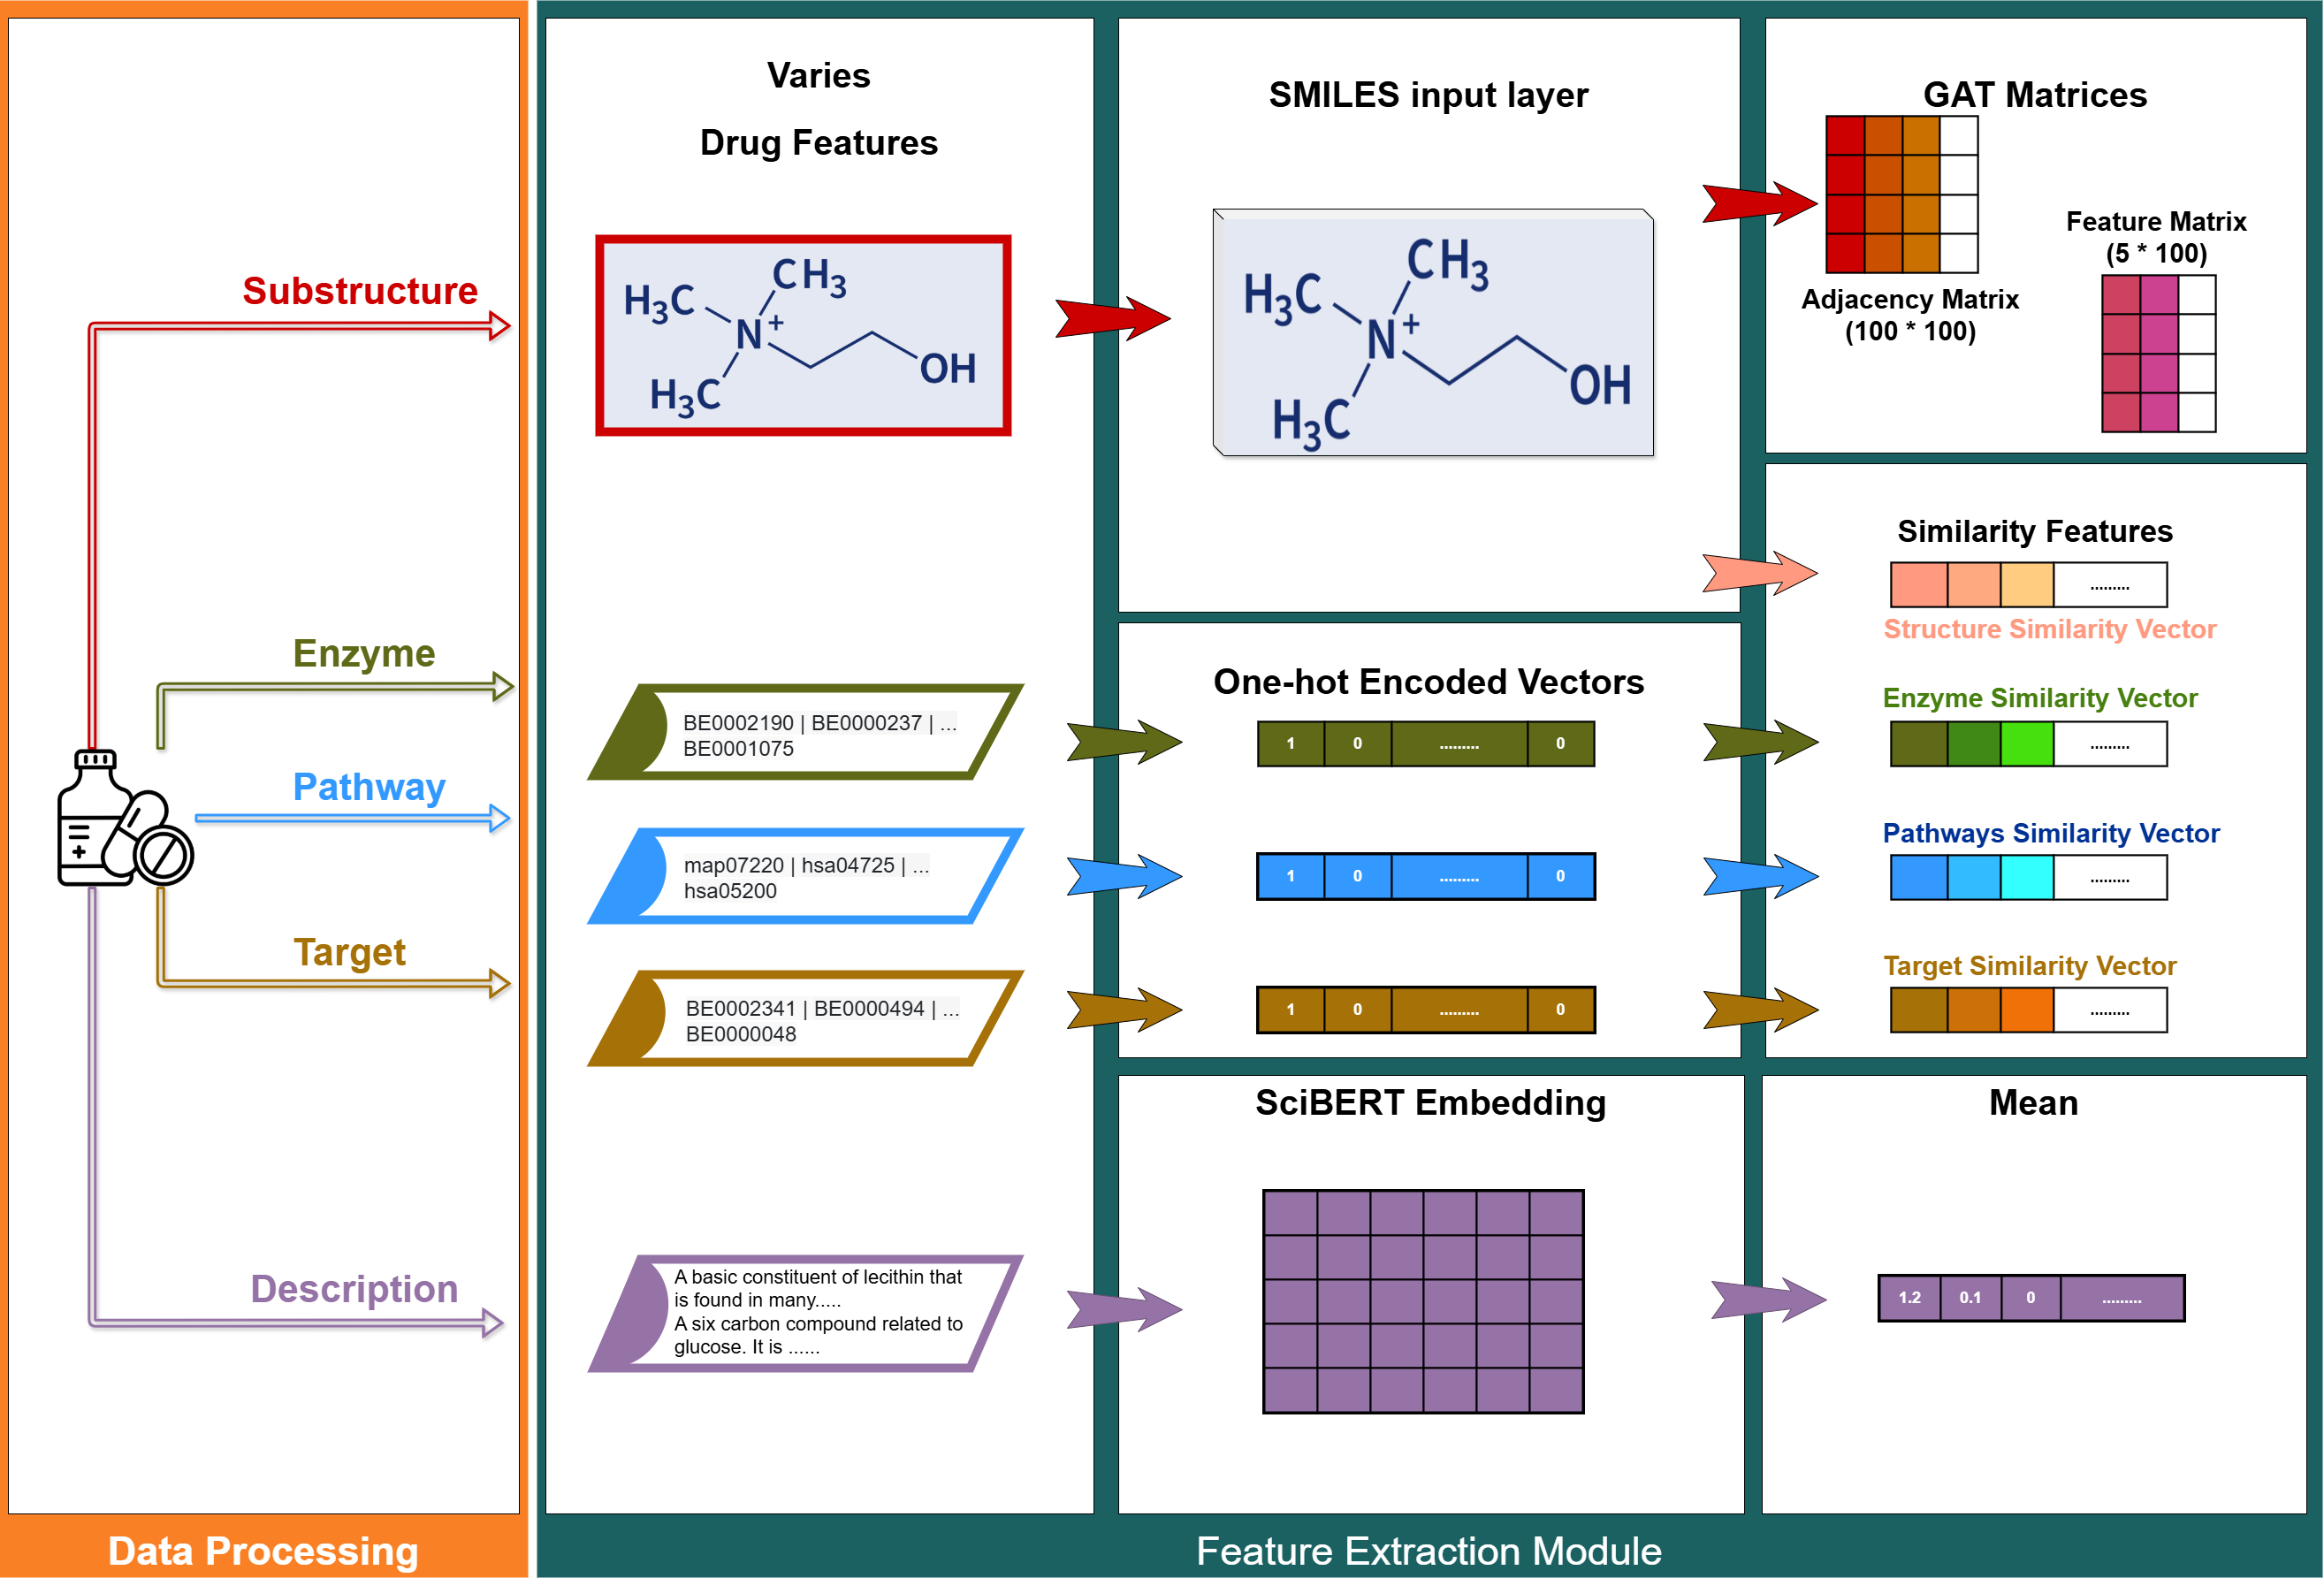
\includegraphics[width=\textwidth]{images/proposed-model-1.png}
		\caption[ ]{مراحل پیش‌پردازش و استخراج ویژگی: تبدیل داده‌های خام به بردارهای ویژگی مختلف}
		\label{fig:sub1}
	\end{subfigure}
	\begin{subfigure}[b]{\textwidth}
		\centering
		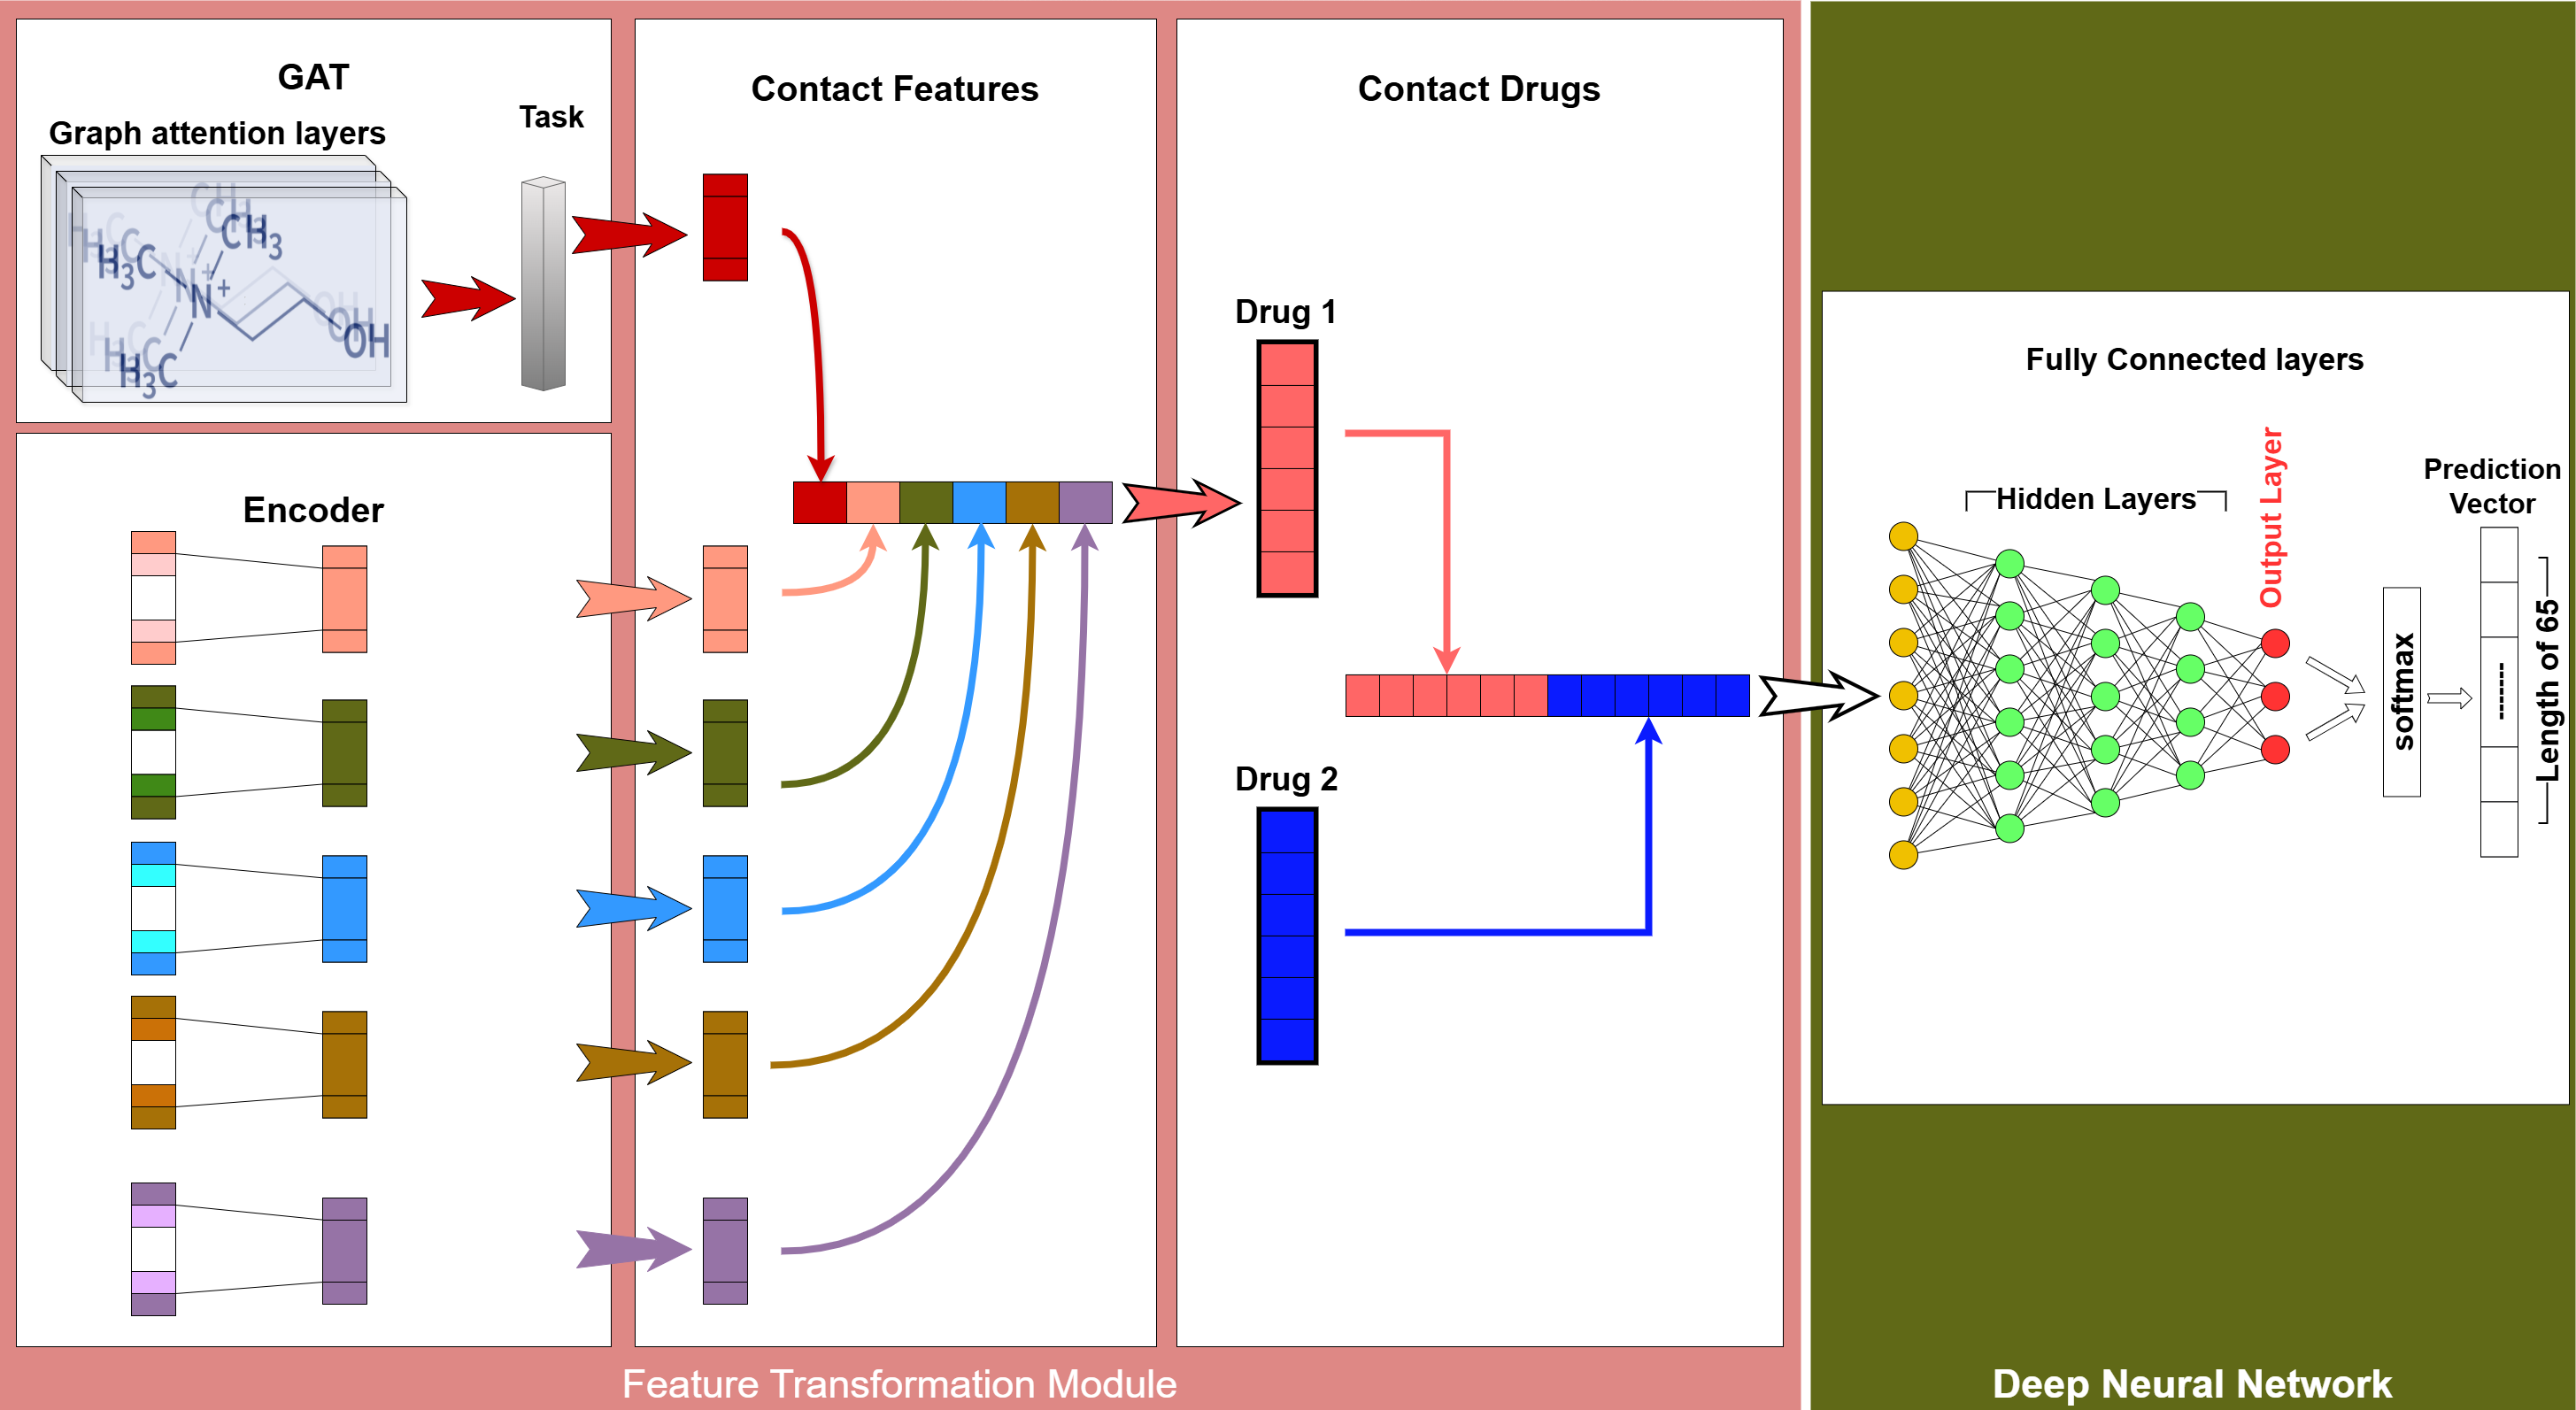
\includegraphics[width=\textwidth]{images/proposed-model-2.png}
		\caption[ ]{معماری شبکه پیش‌بینی: تبدیل و ترکیب ویژگی‌ها و پیش‌بینی نوع تداخل دارویی}
		\label{fig:sub2}
	\end{subfigure}
	\caption{معماری مدل پیشنهادی برای پیش‌بینی تداخلات دارویی} (\subref{fig:sub1}) استخراج و تبدیل ویژگی‌های ساختاری، شباهت و متنی از داده‌های خام، (\subref{fig:sub2}) ترکیب ویژگی‌ها و پیش‌بینی نوع تداخل با استفاده از شبکه عصبی عمیق
	\label{fig:model_architecture}
\end{figure}

بخش دوم مدل که در شکل با عنوان مرحله مبدل ویژگی\LTRfootnote{Feature Transformation} نشان داده شده است، شامل سه مسیر موازی برای استخراج ویژگی‌های مختلف است. مسیر اول با استفاده از یک شبکه عصبی گرافی (\lr{GAT}\LTRfootnote{Graph Attention Network}) به تحلیل ساختار مولکولی داروها می‌پردازد. مسیر دوم با بهره‌گیری از شبکه‌های عصبی پرسپترون چندلایه (\lr{MLP}\LTRfootnote{Multi-Layer Perceptron})، ویژگی‌های شباهت دارویی را پردازش می‌کند. در مسیر سوم، اطلاعات متنی ابتدا توسط مدل زبانی SciBERT تحلیل شده و سپس از طریق یک شبکه عصبی پرسپترون چند لایه پردازش می‌شوند. همانطور که در شکل مشخص است، خروجی این سه مسیر در نهایت با یکدیگر ترکیب می‌شوند تا یک بازنمایی جامع از هر دارو ایجاد شود.

بخش نهایی مدل که در شکل نمایش داده شده است، یک شبکه عصبی عمیق است که بازنمایی‌های نهایی دو دارو را دریافت کرده و با ترکیب آن‌ها، نوع تداخل احتمالی را پیش‌بینی می‌کند. این شبکه که از تکنیک‌های پیشرفته‌ای مانند نرمال‌سازی دسته‌ای\LTRfootnote{Batch Normalization} و حذف تصادفی\LTRfootnote{Dropout} بهره می‌برد، می‌تواند از میان 65 نوع تداخل دارویی شناخته شده، نوع مناسب را با دقت بالا تشخیص دهد.

\section{جمع‌آوری و پیش‌پردازش داده‌ها}

همانطور که در شکل \ref{fig:model_architecture} نشان داده شده است، بخش پردازش داده و استخراج ویژگی در مدل پیشنهادی، شامل پنج مؤلفه اصلی ساختار مولکولی، آنزیم‌ها، مسیرهای بیولوژیکی، اهداف درمانی و توضیحات متنی است. در ادامه، جزئیات نحوه جمع‌آوری و پیش‌پردازش هر یک از این مؤلفه‌ها تشریح می‌شود.

\subsection{منابع داده}

داده‌های مورد نیاز برای این پژوهش عمدتاً از پایگاه داده DrugBank \cite{ref_drugbank} دریافت شدند. DrugBank یک پایگاه داده جامع و به‌روزرسانی شده است که اطلاعات گسترده‌ای در مورد داروها، از جمله ساختار شیمیایی، اهداف درمانی و تداخلات دارویی را فراهم می‌کند. با این حال، به دلیل نقص در بخشی از داده‌های این پایگاه، اطلاعات مربوط به مسیرهای بیولوژیکی از پایگاه داده KEGG \cite{ref_kegg} استخراج شدند. KEGG یک پایگاه داده مرجع برای درک عملکردهای سطح بالاتر سلولی و ارگانیسمی از اطلاعات ژن‌شناختی است. از این دو پایگاه داده، چهار نوع داده اصلی برای هر دارو استخراج شد: ساختار مولکولی، اطلاعات آنزیمی، مسیرهای بیولوژیکی و اهداف درمانی. علاوه بر این، اطلاعات متنی شامل توضیحات\LTRfootnote{Description}، موارد مصرف\LTRfootnote{Indications}، اثرات فارماکودینامیک\LTRfootnote{Pharmacodynamics}، سازوکار عمل\LTRfootnote{Mechanism of action}، اطلاعات مربوط به سمیت\LTRfootnote{Toxicity}، متابولیسم\LTRfootnote{Metabolism}، جذب\LTRfootnote{Absorption}، نیمه‌عمر\LTRfootnote{Half life}، میزان اتصال به پروتئین\LTRfootnote{Protein binding}، مسیرهای حذف\LTRfootnote{Route of elimination} از بدن، حجم توزیع\LTRfootnote{Volume of distribution}، کلیرانس\LTRfootnote{Clearance} و توضیحات طبقه‌بندی\LTRfootnote{Classification description} نیز جمع‌آوری گردید.

برای بازنمایی ساختار مولکولی داروها از کد SMILES استفاده شد که یک استاندارد قابل خواندن توسط ماشین برای نمایش ساختار مولکولی به صورت یک رشته کاراکتری است \cite{ref_weininger1988}. این بازنمایی، اطلاعاتی در مورد اتصالات، پیکربندی، و ایزومری اتم‌ها در یک مولکول را به طور فشرده کدگذاری می‌کند. آنزیم‌ها نقش محوری در متابولیسم داروها و تداخلات دارویی ایفا می‌کنند \cite{ref_cascorbi2012}. این پروتئین‌های تخصصی که به عنوان کاتالیزور عمل می‌کنند، مسئول تبدیل داروها به متابولیت‌های فعال یا غیرفعال هستند. تداخلات دارویی اغلب زمانی رخ می‌دهند که داروها از آنزیم‌های مشترکی برای متابولیسم استفاده می‌کنند یا یک دارو فعالیت آنزیم‌های متابولیزه‌کننده داروی دیگر را تحت تأثیر قرار می‌دهد \cite{ref_huang2013}.

مسیرهای بیولوژیکی مجموعه‌ای از واکنش‌های زنجیره‌ای هستند که عملکردهای حیاتی سلول را کنترل می‌کنند \cite{ref_kegg}. داروها با مداخله در این مسیرها اثرات درمانی خود را اعمال می‌کنند و تداخلات دارویی نیز اغلب در نتیجه تأثیر همزمان داروها بر روی مسیرهای بیولوژیکی مشترک رخ می‌دهد \cite{ref_huang2013}. برای مثال، داروهایی که بر مسیرهای انعقاد خون تأثیر می‌گذارند یا مسیرهای متابولیک کبدی را تحت تأثیر قرار می‌دهند، احتمال بالایی برای ایجاد تداخل با یکدیگر دارند \cite{ref_ryu2018}. اهداف دارویی نیز، که عمدتاً شامل پروتئین‌ها، گیرنده‌ها و آنزیم‌ها هستند، نقش کلیدی در تداخلات دارویی ایفا می‌کنند \cite{ref_drugbank}. تداخلات دارویی اغلب زمانی رخ می‌دهند که داروها اهداف مشترکی داشته باشند یا اثرات متقابلی بر روی اهداف یکدیگر بگذارند \cite{ref_glintborg2005}.

برای استفاده از این داده‌ها در مدل پیش‌بینی، به ازای هر دارو سه بردار ویژگی دودویی مجزا ایجاد شد. برای ساخت بردارهای ویژگی، ابتدا سه فهرست جداگانه شامل تمام آنزیم‌ها، مسیرهای بیولوژیکی و اهداف درمانی از پایگاه داده استخراج شد. سپس برای هر دارو، در هر بردار، حضور (1) یا عدم حضور (0) آن مورد مشخص گردید. در نتیجه، سه بردار ویژگی با ابعاد 325 برای آنزیم‌ها، 405 برای مسیرهای بیولوژیکی و 1613 برای اهداف دارویی به دست آمد. علاوه بر این بردارهای ویژگی، اطلاعات متنی متعددی نیز جمع‌آوری شد که جنبه‌های مختلف داروشناختی و بالینی داروها را پوشش می‌دهند. این مجموعه غنی و چندبعدی از داده‌ها، با ترکیب اطلاعات ساختاری، عملکردی و متنی، امکان کشف ارتباطات پیچیده و الگوهای پنهان در تداخلات دارویی را فراهم می‌کند که با تمرکز بر تعداد محدودی از ویژگی‌ها قابل شناسایی نیستند.

\subsection{طبقه‌بندی تداخلات دارویی}

در این پژوهش، مجموعه داده‌ای شامل 936 دارو مورد استفاده قرار گرفته است. ملاک انتخاب این داروها، در دسترس بودن داده‌های لازم برای استخراج ویژگی‌های مختلف مورد نیاز مدل پیش‌بینی بوده است. این ویژگی‌ها شامل ساختار مولکولی، اهداف درمانی، مسیرهای بیولوژیکی، و آنزیم‌های مرتبط با هر دارو هستند. برای طبقه‌بندی تداخلات بین این داروها، از رویکرد ارائه شده در \cite{ref_ryu2018} استفاده شده است که در آن تداخلات دارویی به 86 دسته تقسیم شده‌اند. با این حال، به دلیل محدودیت‌های موجود در مجموعه داده و برای اطمینان از آموزش مناسب مدل، تنها دسته‌هایی از تداخلات که دارای حداقل 10 نمونه بوده‌اند در نظر گرفته شده‌اند. اعمال این معیار منجر به انتخاب 65 نوع تداخل شده است که به عنوان کلاس‌های هدف در مدل پیش‌بینی مورد استفاده قرار گرفته‌اند. جزئیات کامل این 65 نوع تداخل در پیوست الف ارائه شده است.

انتخاب این طبقه‌بندی چند مزیت کلیدی برای مدل پیشنهادی دارد. اول اینکه این طبقه‌بندی در مطالعات اخیر دیگر نیز مورد استفاده قرار گرفته است \cite{ref_deng2020, ref_asfand2024} که امکان مقایسه مستقیم نتایج را فراهم می‌کند. دوم، تعداد نمونه‌های کافی در هر دسته، امکان آموزش مناسب مدل برای هر نوع تداخل را فراهم می‌آورد. سوم، این دسته‌بندی پوشش مناسبی از انواع مختلف تداخلات دارویی ارائه می‌دهد که برای کاربردهای عملی مدل ضروری است. همچنین استفاده از طبقه‌بندی چندکلاسه با 65 دسته مختلف، مدل را قادر می‌سازد تا علاوه بر تشخیص وجود تداخل بین دو دارو، نوع دقیق آن را نیز مشخص کند.

\subsection{تبدیل SMILES به گراف با استفاده از RDKit}

همانطور که در شکل \ref{fig:model_architecture} نشان داده شده است، برای پردازش ساختار مولکولی داروها، ابتدا باید رشته‌های SMILES به ساختار گرافی تبدیل شوند. این تبدیل منجر به تولید دو ماتریس می‌شود: ماتریس ویژگی‌ها که مشخصات اتم‌ها را نگهداری می‌کند و ماتریس مجاورت\LTRfootnote{Adjacency matrix} که ارتباطات بین اتم‌ها را نشان می‌دهد. برای انجام این تبدیل از کتابخانه RDKit \cite{ref_rdkit} استفاده شده است که یک کتابخانه منبع باز و قدرتمند برای کاربردهای کمو-انفورماتیک و یادگیری ماشین در حوزه داروسازی است. این کتابخانه ابزارهای متنوعی را برای دستکاری، تجزیه و تحلیل و بصری‌سازی ساختارهای مولکولی فراهم می‌کند. فرآیند این تبدیل شامل مراحل زیر است:

\begin{enumerate}
	\item خواندن رشته SMILES برای هر دارو
	\item تبدیل رشته SMILES به یک شیء مولکولی
	\item استخراج اطلاعات اتم‌ها و پیوندها از شیء مولکولی
	\item ساخت ماتریس ویژگی‌های اتمی
	\item ساخت ماتریس مجاورت
\end{enumerate}

در مرحله اول، رشته‌های SMILES که از پایگاه داده DrugBank استخراج شده‌اند، خوانده می‌شوند. سپس هر رشته SMILES به یک شیء مولکولی تبدیل می‌شود. این شیء مولکولی حاوی اطلاعات کاملی در مورد ساختار شیمیایی، اتم‌ها، پیوندها و سایر ویژگی‌های مولکول است. پس از ایجاد شیء مولکولی، دو ماتریس برای بازنمایی ویژگی‌های گرافی مولکول ساخته می‌شوند: ماتریس ویژگی‌های اتمی و ماتریس مجاورت. ماتریس ویژگی‌های اتمی، ویژگی‌های هر اتم را در مولکول ذخیره می‌کند. در این پژوهش، پنج ویژگی اتمی در نظر گرفته شده‌اند:

\begin{enumerate}
	\item عدد اتمی\LTRfootnote{Atomic Number}
	\item درجه اتم\LTRfootnote{Degree} 
	\item بار رسمی اتم\LTRfootnote{Formal Charge}
	\item هیبریداسیون اتم\LTRfootnote{Hybridization}
	\item نشانگر آروماتیک بودن اتم\LTRfootnote{Is Aromatic}
\end{enumerate}

این ویژگی‌ها به ازای هر اتم از مولکول استخراج می‌شوند و در ماتریسی با ابعاد $N \times 5$ ذخیره می‌شوند، که $N$ تعداد اتم‌های موجود در مولکول است. برای یکسان‌سازی ابعاد ورودی و کارایی محاسباتی، تعداد اتم‌های در نظر گرفته شده برای هر مولکول به 100 محدود شده است. مولکول‌هایی با بیش از 100 اتم، فقط 100 اتم اول آنها در نظر گرفته می‌شوند، در حالی که برای مولکول‌های کوچکتر، ردیف‌های خالی در ماتریس ویژگی با صفر پر می‌شوند. علاوه بر ماتریس ویژگی‌های اتمی که اطلاعات مربوط به هر اتم را در خود ذخیره می‌کند، ارتباطات میان اتم‌ها در مولکول نیز مورد توجه قرار می‌گیرد. ماتریس مجاورت که این ارتباطات را نشان می‌دهد، یک ماتریس متقارن با ابعاد $100 \times 100$ است. درایه $(i,j)$ این ماتریس نشان می‌دهد آیا اتم $i$ و اتم $j$ در مولکول با هم پیوند دارند یا خیر.

این دو ماتریس (ویژگی‌های اتمی و مجاورت) به عنوان بازنمایی‌های گرافی از ساختار مولکولی هر دارو در مراحل بعدی مدل مورد استفاده قرار می‌گیرند و به ترتیب به عنوان ماتریس ویژگی‌های گره و ماتریس ارتباطات در یک گراف در نظر گرفته می‌شوند. این رویکرد استخراج ویژگی مبتنی بر گراف، امکان بهره‌گیری از اطلاعات ساختاری غنی موجود در بازنمایی ساختار مولکولی داروها را در مدل پیش‌بینی تداخل فراهم می‌کند. با تعبیه ساختار مولکولی در فضای گرافی، می‌توان الگوهای پنهان و وابستگی‌های ساختاری مرتبط با تداخلات دارویی را آشکار کرد و برای بهبود دقت پیش‌بینی‌ها استفاده نمود.

\subsection{پیش‌پردازش ویژگی‌های شباهت دارویی}


همانطور که در شکل \ref{fig:model_architecture} نشان داده شده است، برای درک عمیق‌تر روابط بین داروها، شباهت‌های چندگانه بین آن‌ها بر اساس چهار دیدگاه اصلی محاسبه شده است: ساختار مولکولی، اهداف درمانی، آنزیم‌های مرتبط و مسیرهای بیولوژیکی. برای محاسبه این شباهت‌ها، معیارهای مختلفی مورد ارزیابی قرار گرفتند که در نهایت معیار Jaccard به دلیل عملکرد بهتر در پیش‌بینی تداخلات دارویی انتخاب شد. این یافته با نتایج مطالعات پیشین نیز همخوانی دارد؛ برای مثال، \cite{ref_kumari2024} نشان داد که معیار Jaccard در مقایسه با سایر معیارهای شباهت مانند \lr{Cosine}، همبستگی بیشتری با الگوهای تداخلات دارویی دارد. معیار Jaccard که یک روش قدرتمند برای مقایسه مجموعه‌ها و تعیین میزان همپوشانی آن‌هاست، به صورت نسبت اندازه اشتراک دو مجموعه به اندازه اجتماع آن‌ها تعریف می‌شود:

\begin{equation}
	J(A,B) = \frac{|A \cap B|}{|A \cup B|}
\end{equation}

در این فرمول، $A$ و $B$ مجموعه‌های باینری مورد مقایسه هستند، $|A \cap B|$ نشان‌دهنده تعداد مواردی است که در هر دو مجموعه با یک مقداردهی شده‌اند (عناصر مشترک با مقدار 1) و $|A \cup B|$ بیانگر تعداد کل مواردی است که حداقل در یکی از دو مجموعه با یک مقداردهی شده‌اند (مجموع عناصر با مقدار 1، بدون شمارش مجدد عناصر مشترک). مقدار این ضریب همواره بین 0 و 1 قرار دارد، به طوری که مقدار 1 نشان‌دهنده شباهت کامل (دو مجموعه کاملاً یکسان) و مقدار 0 بیانگر عدم وجود هیچ شباهتی (دو مجموعه کاملاً متمایز) است. این معیار به دلیل سادگی محاسبه و تفسیر آسان، به طور گسترده در مقایسه مجموعه‌های باینری مورد استفاده قرار می‌گیرد.

برای محاسبه شباهت ساختار مولکولی، از کتابخانه RDKit استفاده شده است. این کتابخانه امکان مقایسه دقیق ساختارهای مولکولی را از طریق تحلیل رشته‌های SMILES فراهم می‌کند. در این فرآیند، ابتدا ساختار مولکولی هر دارو بازسازی شده و سپس با استفاده از توابع تخصصی \lr{RDKit}، زیرساختارهای مشترک بین مولکول‌ها شناسایی و مقایسه می‌شوند.

برای محاسبه شباهت‌های عملکردی (اهداف درمانی، آنزیم‌ها و مسیرهای بیولوژیکی)، یک رویکرد نظام‌مند طراحی شده است. در این رویکرد، ابتدا برای هر نوع ویژگی، یک ماتریس دودویی با ابعاد $N \times M$ ایجاد می‌شود که $N$ تعداد داروها (936) و $M$ تعداد مقادیر منحصر به فرد آن نوع ویژگی است. برای هر دارو $i$، اگر ویژگی $j$ برای آن صدق کند، درایه متناظر $(i,j)$ در ماتریس برابر 1 و در غیر این صورت برابر 0 قرار می‌گیرد. پس از تشکیل این ماتریس دودویی، ضریب شباهت Jaccard بین هر جفت دارو محاسبه می‌شود. این محاسبات در نهایت به یک ماتریس شباهت $N \times N$ منجر می‌شود که درایه $(i,j)$ آن نشان‌دهنده میزان شباهت بین داروی $i$ و داروی $j$ از نظر آن نوع ویژگی است.

در نهایت، این فرآیند منجر به تولید چهار ماتریس شباهت متمایز می‌شود که هر کدام از زاویه‌ای متفاوت، روابط بین داروها را توصیف می‌کنند. همانطور که در شکل \ref{fig:model_architecture}-\subref{fig:sub1} نشان داده شده است، این ماتریس‌های شباهت در مرحله مبدل ویژگی با سایر ویژگی‌های استخراج شده ترکیب می‌شوند تا بازنمایی جامعی از هر دارو ایجاد شود. ترکیب این شباهت‌های چندگانه، مدل را قادر می‌سازد تا الگوهای پیچیده و پنهان در تداخلات دارویی را با دقت بیشتری شناسایی کند و عملکرد بهتری در پیش‌بینی انواع مختلف تداخلات داشته باشد.

فرآیند پیش‌پردازش ویژگی‌های شباهت دارویی، گامی اساسی در آماده‌سازی داده‌ها برای استفاده در مدل پیش‌بینی تداخل دارویی است. این ویژگی‌های جدید، اطلاعات ارزشمندی را در مورد ارتباطات بین داروها بر اساس خواص ساختاری و عملکردی آنها فراهم می‌کنند و می‌توانند به بهبود عملکرد و تعمیم‌پذیری مدل کمک کنند. با این حال، این رویکرد محدودیت‌هایی نیز دارد. مهم‌ترین چالش، افزودن داروهای جدید به سامانه است؛ زیرا برای هر داروی جدید، باید شباهت آن با تمام داروهای موجود محاسبه شده و ماتریس شباهت به‌روزرسانی شود. این فرآیند می‌تواند از نظر محاسباتی پرهزینه باشد، به خصوص زمانی که تعداد داروها زیاد است. علاوه بر این، برای داروهای جدیدی که اطلاعات کافی در مورد اهداف، آنزیم‌ها یا مسیرهای بیولوژیکی آنها در دسترس نیست، محاسبه دقیق شباهت‌ها می‌تواند چالش‌برانگیز باشد.

\subsection{تبدیل ویژگی‌های متنی با استفاده از SciBERT}

همانطور که در بخش پایینی شکل \ref{fig:model_architecture}-\subref{fig:sub1} نشان داده شده است، علاوه بر ویژگی‌های ساختاری و شباهت، از اطلاعات متنی استخراج شده از پایگاه‌های داده برای غنی‌سازی بازنمایی داروها استفاده شده است. برای استخراج نمایش عددی\LTRfootnote{Embedding} معنادار از این داده‌های متنی، از مدل SciBERT استفاده شده است که یک مدل زبانی پیش‌آموزش دیده بر اساس معماری BERT \cite{ref_devlin2018} است و به طور خاص برای متون علمی و فنی بهینه‌سازی شده است. این مدل با استفاده از سازوکار توجه دوطرفه\LTRfootnote{Bidirectional Attention} و آموزش بر روی مجموعه‌ای بزرگ از مقالات علمی و پزشکی، توانایی درک عمیق اصطلاحات تخصصی، ساختارهای نحوی و روابط معنایی در متون علمی را دارد \cite{ref_beltagy2019}. مزیت اصلی SciBERT نسبت به مدل BERT پایه، درک بهتر متون تخصصی و علمی است که آن را برای پردازش متون دارویی بسیار مناسب می‌سازد.

فرآیند تبدیل ویژگی‌های متنی با استفاده از SciBERT با پیش‌پردازش متن آغاز می‌شود. در این مرحله، متن مربوط به هر ویژگی دارویی استخراج شده و عملیات نرمال‌سازی مانند حذف علائم نگارشی اضافی، یکسان‌سازی قالب کاراکترها و تبدیل به حروف کوچک انجام می‌شود. سپس متن به توکن‌های کوچکتر شکسته می‌شود. SciBERT از یک توکن‌ساز تخصصی استفاده می‌کند که بر اساس الگوریتم WordPiece آموزش دیده و می‌تواند اصطلاحات تخصصی علمی را به درستی تشخیص دهد.

در مرحله بعد، توکن‌های پیش‌پردازش شده به مدل SciBERT تغذیه می‌شوند. مدل برای هر توکن، یک بردار نهان\LTRfootnote{Hidden state} با ابعاد 768 تولید می‌کند که حاوی اطلاعات معنایی و زمینه‌ای آن توکن است. این بردارها با استفاده از سازوکار توجه چندلایه‌ای SciBERT تولید می‌شوند که به مدل اجازه می‌دهد ارتباطات پیچیده بین کلمات را در نظر بگیرد. با توجه به محدودیت طول ورودی SciBERT که حداکثر 512 توکن را می‌پذیرد و اینکه تنها تعداد اندکی از متون از این محدودیت فراتر می‌رفتند، برای این موارد محدود، 512 توکن اول در نظر گرفته شد. سپس برای تولید یک بازنمایی یکپارچه، بردارهای نهان تولید شده برای توکن‌ها با استفاده از عملگر میانگین‌گیری لایه آخر\LTRfootnote{Last layer mean pooling} با هم ترکیب می‌شوند که منجر به تولید یک بردار 768 بعدی می‌شود که نمایانگر معنای کلی متن است.

در نهایت، بردارهای نمایش به دست آمده از تمام ویژگی‌های متنی یک دارو با یکدیگر ترکیب شده و یک بردار ویژگی جامع برای آن دارو تشکیل می‌دهند. این بردار نهایی، که اطلاعات غنی متنی را در خود جای داده است، در کنار سایر ویژگی‌های استخراج شده (مانند ویژگی‌های ساختاری و شباهت) قرار می‌گیرد تا بازنمایی کاملی از دارو ایجاد شود که می‌تواند برای پیش‌بینی تداخلات دارویی مورد استفاده قرار گیرد.

بهره‌گیری از SciBERT در این پژوهش، امکان استخراج اطلاعات معنادار از داده‌های متنی غیرساختاریافته را فراهم می‌کند. این مدل با درک عمیق متون علمی و پزشکی، می‌تواند نکات ظریف و روابط پیچیده موجود در توصیفات دارویی را شناسایی کند. ترکیب این اطلاعات معنایی با سایر ویژگی‌های دارویی، به بهبود قابل توجه دقت و قدرت تعمیم مدل پیش‌بینی تداخل دارویی کمک می‌کند.

\section{ویژگی‌ها و معماری مدل پیشنهادی}

در این بخش، جزئیات مربوط به ویژگی‌های مورد استفاده و معماری مدل پیشنهادی برای پیش‌بینی تداخلات دارویی ارائه می‌شود. همانطور که در شکل \ref{fig:model_architecture} نشان داده شد، مدل پیشنهادی یک رویکرد جامع و چندوجهی را دنبال می‌کند که از انواع مختلف داده‌های دارویی، از جمله ساختار مولکولی، شباهت‌های عملکردی، و اطلاعات متنی استفاده می‌کند. هدف این مدل، استخراج ویژگی‌های غنی و بازنمایی‌های عمیق از داروها برای پیش‌بینی دقیق تداخلات دارویی است. در ادامه، هر یک از بخش‌های این معماری با جزئیات بیشتر تشریح می‌شوند.

\subsection{مدل استخراج ویژگی و ادغام ویژگی‌ها}

همانطور که در شکل \ref{fig:model_architecture}-\subref{fig:sub2} نشان داده شده است، پس از پیش‌پردازش و تبدیل داده‌های خام دارویی به قالب‌های مناسب، بردارهای ویژگی اولیه حاصل از بخش‌های مختلف (ساختاری، شباهت، و متنی) وارد مرحله مبدل ویژگی می‌شوند. در این مرحله، مدل‌های یادگیری عمیق مانند شبکه‌های توجه گراف برای پردازش ویژگی‌های ساختاری و شبکه‌های عصبی پرسپترون چندلایه برای پردازش ویژگی‌های شباهت و متنی مورد استفاده قرار می‌گیرند. هدف این مرحله، استخراج بازنمایی‌های عمیق‌تر و غنی‌تر از ویژگی‌های اولیه است. پس از اتمام مرحله مبدل ویژگی، همانطور که در شکل نشان داده شده است، بردارهای ویژگی پردازش شده برای هر دارو در مرحله ادغام ویژگی\LTRfootnote{Feature Concatenation} در کنار هم قرار می‌گیرند تا یک بردار ویژگی یکپارچه برای آن دارو ایجاد شود. در نهایت، در مرحله ادغام دارو\LTRfootnote{Drug Concatenation}، بردارهای ویژگی نهایی برای هر دو داروی مورد بررسی با هم ترکیب می‌شوند تا ورودی نهایی برای شبکه عصبی پیش‌بینی کننده تداخلات دارویی آماده شود.


\subsection{جزئیات شبکه توجه گراف در بخش ساختاری}

همانطور که در شکل \ref{fig:model_architecture}-\subref{fig:sub2} نشان داده شده است، در بخش پردازش ویژگی‌های ساختاری مولکولی، از یک مدل شبکه توجه گراف برای استخراج بازنمایی‌های گرافی از ساختار مولکولی داروها استفاده می‌شود. مدل شبکه توجه گراف، یک نوع شبکه عصبی گرافی است که از سازوکار توجه\LTRfootnote{Attention} برای وزن‌دهی به اهمیت گره‌های مختلف در گراف استفاده می‌کند.

معماری شبکه توجه گراف (GAT) شامل یک لایه تبدیل خطی برای پردازش ویژگی‌های گره‌ها و یک مکانیزم محاسبه وزن‌های توجه است. ابتدا ویژگی‌های گره‌ها و ساختار گراف (بر اساس ماتریس مجاورت) به عنوان ورودی دریافت می‌شوند. سپس، یک تبدیل خطی روی ویژگی‌های گره‌ها اعمال شده و ضرایب توجه برای هر گره در ارتباط با گره‌های همسایه محاسبه می‌گردد. پس از محاسبه ضرایب توجه، تابع LeakyReLU برای افزایش غیرخطی بودن اعمال شده و سپس با استفاده از تابع Softmax، این ضرایب نرمال‌سازی می‌شوند. این ضرایب نرمال شده، اهمیت نسبی هر گره را در گراف نشان می‌دهند. پس از اعمال وزن‌های توجه بر روی ویژگی‌های تبدیل یافته، یک میانگین‌گیری روی گره‌ها انجام می‌شود تا بازنمایی نهایی گراف به دست آید. این بازنمایی نهایی که اندازه آن 64 بعدی است، حاوی اطلاعات ساختاری غنی از مولکول‌های دارویی است و به عنوان ورودی به شبکه پیش‌بینی کننده تداخلات دارویی داده می‌شود.

شکل \ref{fig:gat_model} جزئیات معماری مدل شبکه توجه گراف مورد استفاده در این بخش را نشان می‌دهد. استفاده از این معماری در پژوهش حاضر، امکان استخراج بازنمایی‌های ساختاری قدرتمند و انعطاف‌پذیر از مولکول‌های دارویی را فراهم می‌کند. این بازنمایی‌ها، اطلاعات مهمی در مورد ارتباطات و اهمیت نسبی اجزای ساختاری مولکول‌ها را در اختیار مدل پیش‌بینی تداخلات دارویی قرار می‌دهند و به بهبود عملکرد آن کمک می‌کنند.

\begin{figure}[!t]
	\centering
	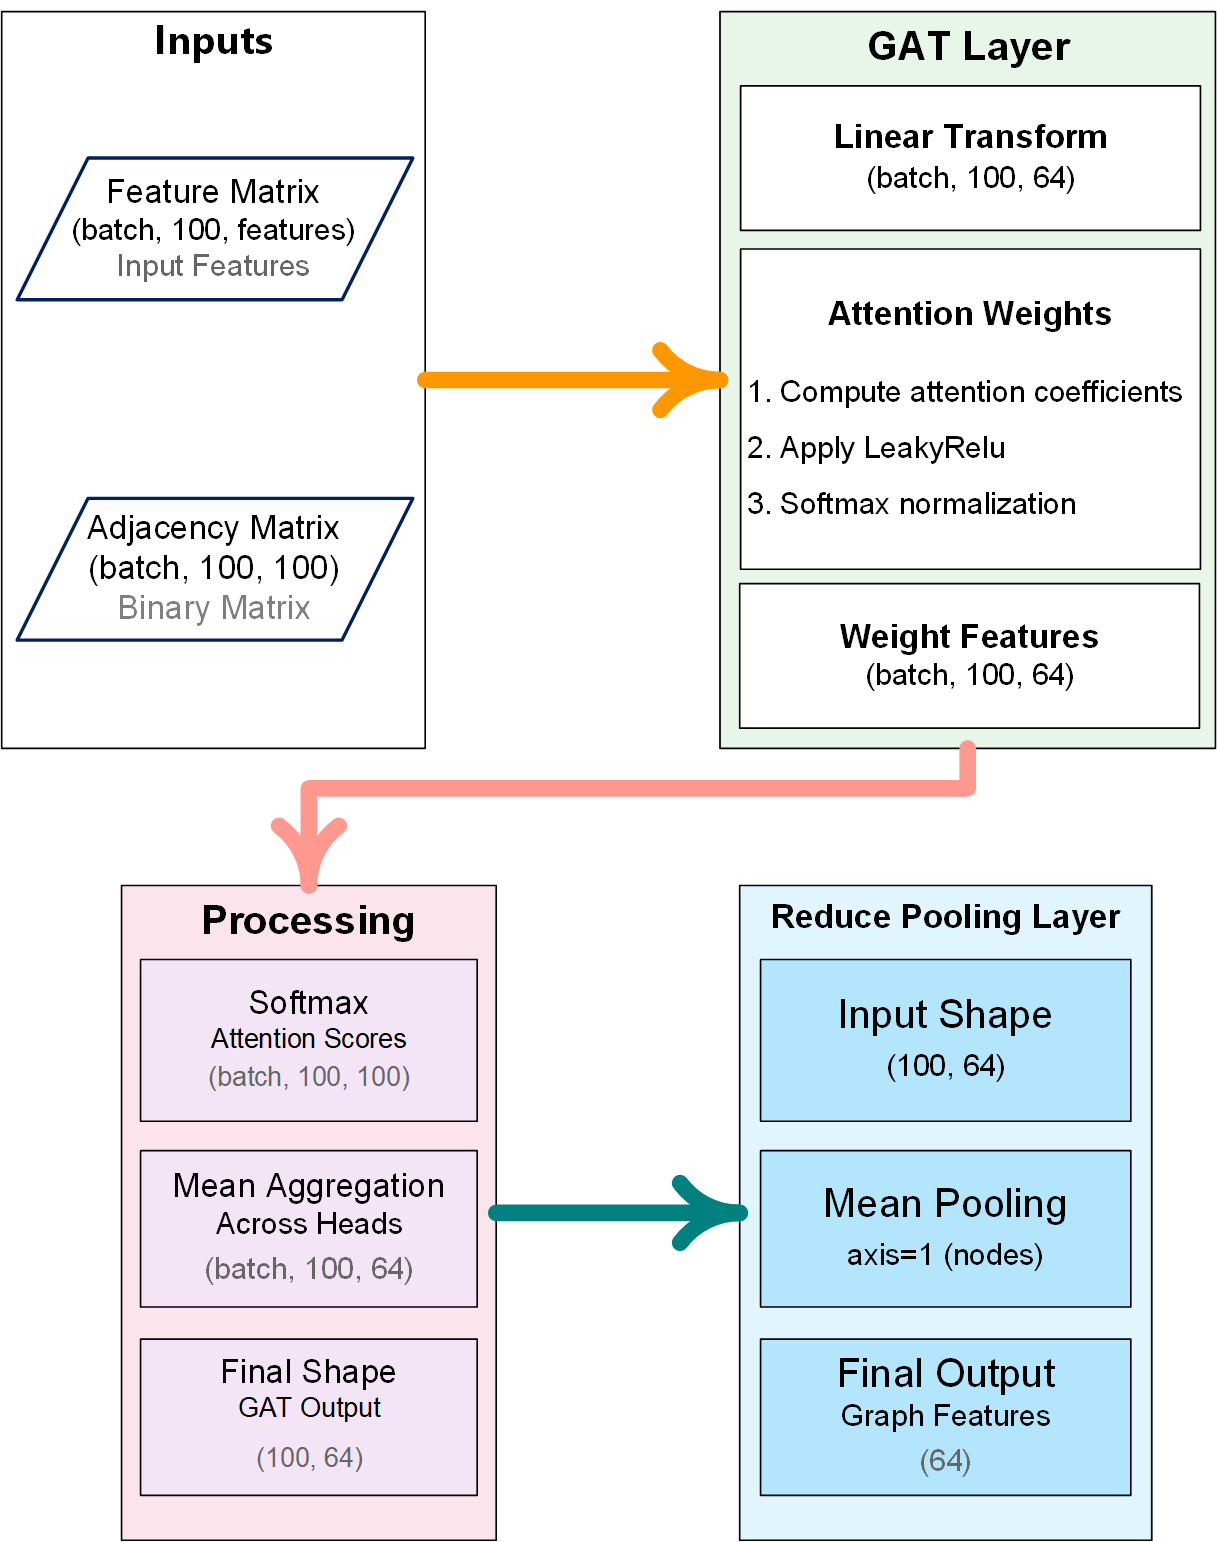
\includegraphics[width=0.8\textwidth]{images/gat-model.png}
	\caption{معماری مدل شبکه توجه گراف مورد استفاده در بخش پردازش ویژگی‌های ساختاری}
	\label{fig:gat_model}
\end{figure}

\subsection{جزئیات شبکه‌ پرسپترون چندلایه در بخش‌های شباهت و متنی}

همانطور که در شکل \ref{fig:model_architecture}-\subref{fig:sub2} در بخش مبدل ویژگی نشان داده شده است، در بخش‌های پردازش ویژگی‌های شباهت دارویی و ویژگی‌های متنی، از شبکه‌های عصبی پرسپترون چندلایه برای تبدیل بازنمایی‌های اولیه به فضاهای ویژگی فشرده‌تر و معنادارتر استفاده می‌شود. برای هر نوع ویژگی شباهت (مانند شباهت ساختاری، شباهت مسیرهای بیولوژیکی، شباهت اهداف، و شباهت آنزیم‌ها) و هر ویژگی متنی، یک پرسپترون چندلایه مجزا با معماری خاص طراحی شده است. این شبکه‌های عصبی از لایه‌های متراکم\LTRfootnote{Dense} با تعداد واحدهای کمتر نسبت به ابعاد ورودی و توابع فعال‌سازی غیرخطی (مانند \LR{ReLU}) تشکیل شده‌اند. هدف اصلی این معماری، کاهش ابعاد داده‌ها و استخراج ویژگی‌های سطح بالاتر از بازنمایی‌های ورودی است.

مدل با استفاده از این معماری قادر است ویژگی‌های مهم و مرتبط را از ماتریس‌های شباهت و بردارهای ویژگی متنی استخراج کند و آنها را به بازنمایی‌های فشرده‌تر تبدیل نماید. این بازنمایی‌های فشرده، ضمن حفظ اطلاعات اصلی، به کاهش پیچیدگی محاسباتی شبکه کمک می‌کنند. در طراحی این مدل، برای افزایش کارایی از راهبرد اشتراک پارامترها استفاده شده است؛ به این معنی که برای هر نوع ویژگی، شبکه‌های عصبی مربوط به دو داروی مورد مقایسه از پارامترهای یکسانی استفاده می‌کنند. برای مثال، شبکه عصبی مربوط به شباهت ساختاری برای هر دو دارو یکسان است. این رویکرد به مدل اجازه می‌دهد تا الگوهای مشابه را در ویژگی‌های مشترک دو دارو بهتر شناسایی کند.

نتیجه نهایی فرآیند پردازش، ترکیب خروجی‌های شبکه‌های عصبی پرسپترون چندلایه با خروجی بخش شبکه توجه گراف (بازنمایی ساختار مولکولی) در بخش ادغام ویژگی‌ها\LTRfootnote{Feature Concatenation} است. این ترکیب، بازنمایی نهایی و جامعی از هر دارو را قبل از ورود به بخش پیش‌بینی تداخل دارویی فراهم می‌کند. استفاده از معماری شبکه عصبی پرسپترون چندلایه در بخش‌های شباهت و متنی مدل پیشنهادی، علاوه بر استخراج ویژگی‌های مرتبط‌تر و فشرده‌تر از داده‌های ورودی، به بهبود کارایی محاسباتی و عملکرد پیش‌بینی مدل نیز کمک می‌کند. این رویکرد نشان‌دهنده اهمیت استفاده از سازوکار‌های کاهش ابعاد و استخراج ویژگی در معماری‌های یادگیری عمیق برای تحلیل داده‌های پیچیده دارویی است.

\subsection{پیش‌بینی تداخل دارویی}

همانطور که در شکل \ref{fig:model_architecture}-\subref{fig:sub2} نشان داده شده است، پس از ادغام ویژگی‌های استخراج شده از بخش‌های مختلف مدل، بازنمایی نهایی هر جفت دارو وارد مرحله پیش‌بینی تداخل دارویی می‌شود. در این مرحله، که در شکل به صورت یک شبکه عصبی کاملاً متصل\LTRfootnote{Fully Connected Neural Network} نمایش داده شده است، از یک معماری عمیق و پیچیده برای پیش‌بینی نوع تداخل دارویی استفاده شده است \cite{ref_dai2020}. این شبکه با هدف مدل‌سازی روابط پیچیده و غیرخطی بین ویژگی‌های داروها طراحی شده و قادر است با دقت بالایی نوع تداخل احتمالی را پیش‌بینی نماید.

معماری شبکه عصبی پیش‌بینی کننده از یک ساختار کاهشی بهره می‌برد که شامل چندین لایه متراکم متوالی است. این معماری با سه لایه متراکم طراحی شده که به ترتیب دارای 1024، 512 و 256 نورون هستند. کاهش تدریجی در تعداد نورون‌ها یک راهبرد حساب شده است که به مدل اجازه می‌دهد در هر مرحله، اطلاعات مهم‌تر را از فضای ویژگی استخراج کرده و بازنمایی‌های فشرده‌تر و معنادارتری ایجاد کند. این رویکرد کاهشی همچنین به کنترل پیچیدگی مدل و جلوگیری از بیش‌برازش کمک می‌کند.

برای افزایش کارایی و پایداری آموزش شبکه، پس از هر لایه متراکم از مجموعه‌ای از تکنیک‌های بهینه‌سازی استفاده شده است. نرمال‌سازی دسته‌ای با نرمال‌سازی توزیع خروجی هر لایه، سرعت همگرایی شبکه را افزایش می‌دهد و وابستگی به مقداردهی اولیه پارامترها را کاهش می‌دهد \cite{ref_dai2020}. تابع فعال‌سازی ReLU با معرفی غیرخطی به شبکه، توانایی مدل‌سازی روابط پیچیده را افزایش می‌دهد و مشکل محو شدن گرادیان را که در توابع فعال‌سازی سنتی مانند \lr{tanh} رایج است، برطرف می‌کند. همچنین، تکنیک حذف تصادفی با نرخ \lr{0.3} پس از هر لایه اعمال می‌شود که با غیرفعال کردن تصادفی برخی نورون‌ها در حین آموزش، از وابستگی بیش از حد مدل به ویژگی‌های خاص جلوگیری می‌کند و قابلیت تعمیم آن را افزایش می‌دهد.

در لایه نهایی، از یک تابع فعال‌سازی بیشینه هموار\LTRfootnote{Softmax} با 65 نورون (متناسب با تعداد انواع تداخلات) استفاده شده است. این لایه برای هر نوع تداخل دارویی، یک احتمال بین 0 تا 1 تولید می‌کند، به طوری که مجموع تمام احتمالات برابر 1 است. تابع بیشینه هموار با تبدیل خروجی‌های خام شبکه به توزیع احتمال، امکان تفسیر بهتر نتایج را فراهم می‌کند. در نهایت، نوع تداخلی که بالاترین احتمال را به خود اختصاص داده است، به عنوان پیش‌بینی نهایی مدل انتخاب می‌شود.

این معماری عمیق و چندلایه با ترکیب هوشمندانه تکنیک‌های مختلف بهینه‌سازی و تنظیم، قادر است الگوهای پیچیده در داده‌های ورودی را شناسایی کند و پیش‌بینی‌های دقیقی از نوع تداخل دارویی ارائه دهد. استفاده از لایه‌های تنظیم‌کننده مانند حذف تصادفی و نرمال‌سازی دسته‌ای نه تنها پایداری و تعمیم‌پذیری مدل را در مواجهه با داده‌های جدید تضمین می‌کند، بلکه با بهبود فرآیند آموزش، به دستیابی سریع‌تر به همگرایی نیز کمک می‌کند. این ویژگی‌ها در مجموع، مدل را برای کاربرد در محیط‌های واقعی و مواجهه با داده‌های نویزدار مناسب می‌سازد

\subsection{مزایای اشتراک‌گذاری پارامترها در بهبود عملکرد مدل}

یکی از ویژگی‌های کلیدی مدل پیشنهادی، استفاده از پارامترهای مشترک\LTRfootnote{Shared parameters} در شبکه‌های عصبی پردازش‌کننده دو داروی ورودی است. در این رویکرد، به جای استفاده از شبکه‌های مجزا برای هر دارو، از یک شبکه واحد با پارامترهای مشترک استفاده می‌شود که مزایای قابل توجهی در بهبود عملکرد و کارایی مدل دارد \cite{ref_dai2020}. برای درک بهتر این مفهوم کلیدی، در شکل \ref{fig:param_sharing} نمای شماتیکی از نحوه اشتراک‌گذاری پارامترها در بخش‌های مختلف مدل نشان داده شده است. این شکل به خوبی نشان می‌دهد چگونه شبکه‌های پردازشی یکسان برای استخراج ویژگی‌های متناظر در هر دو دارو استفاده می‌شوند.

\begin{figure}[t]
	\centering
	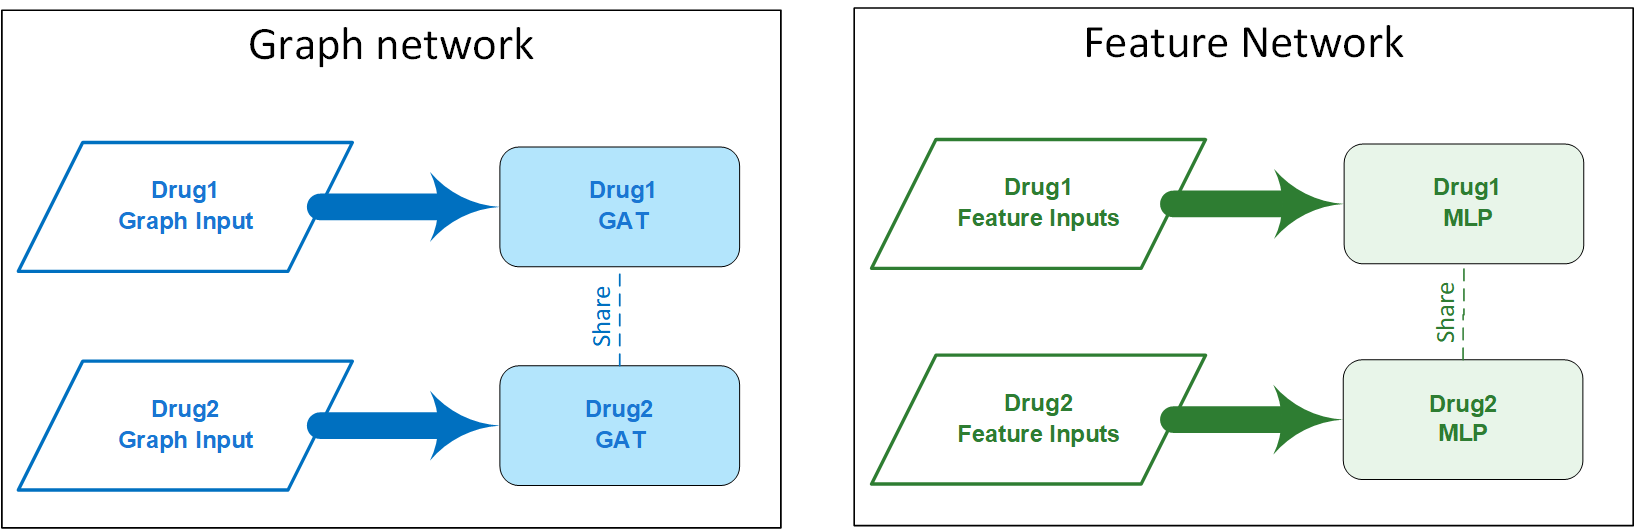
\includegraphics[width=\textwidth]{images/param-sharing.png}
	\caption{نمایش شماتیک اشتراک‌گذاری پارامترها در مدل پیشنهادی} استفاده از وزن‌های مشترک در شبکه‌های گراف و شبکه‌های ویژگی برای پردازش هر دو دارو
	\label{fig:param_sharing}
\end{figure}

اشتراک‌گذاری پارامترها به مدل امکان می‌دهد الگوهای مشترک و روابط بین داروها را با دقت بیشتری شناسایی کند. از آنجا که هر دو دارو توسط یک شبکه واحد پردازش می‌شوند، دانش کسب شده از تحلیل یک دارو می‌تواند مستقیماً در تحلیل داروی دیگر مورد استفاده قرار گیرد. این انتقال دانش به مدل کمک می‌کند تا از اطلاعات موجود در هر دو دارو برای پیش‌بینی دقیق‌تر تداخلات دارویی استفاده کند \cite{ref_deng2020}.

یکی دیگر از مزایای مهم این رویکرد، کمک به جلوگیری از بیش‌برازش از طریق کاهش پیچیدگی مدل است \cite{ref_xu2019}. با محدود کردن تعداد پارامترهای مستقل، احتمال یادگیری الگوهای تصادفی و نویز در داده‌های آموزشی کاهش می‌یابد. این ویژگی به خصوص در مواجهه با داده‌های جدید و دیده نشده اهمیت پیدا می‌کند، زیرا مدل با تکیه بر الگوهای اساسی و معنادار، قابلیت تعمیم بهتری پیدا می‌کند.

اشتراک‌گذاری پارامترها همچنین تأثیر قابل توجهی بر کارایی محاسباتی مدل دارد. با کاهش تعداد کل پارامترهای مدل، این رویکرد باعث صرفه‌جویی چشمگیر در حافظه مورد نیاز می‌شود. در مدل پیشنهادی، استفاده از پارامترهای مشترک در شبکه‌های توجه گراف و پرسپترون چندلایه تعداد پارامترهای مدل را تقریباً به نصف کاهش داده است \cite{ref_dai2020}. این کاهش در تعداد پارامترها مزایای عملی متعددی به همراه دارد. از جمله این مزایا می‌توان به افزایش سرعت همگرایی مدل اشاره کرد، زیرا تعداد پارامترهای کمتری باید در هر تکرار به‌روزرسانی شوند. همچنین، زمان آموزش مدل کاهش می‌یابد که در کاربردهای عملی بسیار حائز اهمیت است.

در مجموع، اشتراک‌گذاری پارامترها یکی از جنبه‌های کلیدی معماری مدل پیشنهادی است که با کاهش پیچیدگی محاسباتی، بهبود قابلیت تعمیم، و امکان اجرا روی سخت‌افزارهای متنوع، نقش مهمی در کاربردی کردن مدل ایفا می‌کند. این رویکرد نه تنها به دستیابی به پیش‌بینی‌های دقیق‌تر کمک می‌کند، بلکه امکان استفاده گسترده‌تر از مدل در محیط‌های با محدودیت منابع را نیز فراهم می‌آورد.

\subsection{چالش‌ها و نوآوری‌های مدل پیشنهادی}

پیچیدگی و چندوجهی بودن مدل پیشنهادی چالش‌های متعددی را در مسیر طراحی و پیاده‌سازی آن ایجاد کرده است. یکی از اساسی‌ترین این چالش‌ها، مدیریت حجم بالای داده‌ها و ابعاد زیاد ویژگی‌های ورودی است. در حالی که اکثر روش‌های موجود بر روی داده‌های ساختاری و عملکردی داروها تمرکز کرده‌اند \cite{ref_deng2020, ref_shi2024}، مدل پیشنهادی همانطور که در شکل \ref{fig:model_architecture}-\subref{fig:sub1} نشان داده شده است، علاوه بر ساختار مولکولی، اطلاعات آنزیمی، مسیرهای بیولوژیکی و اهداف درمانی، از داده‌های متنی غنی نیز برای درک جامع‌تر ویژگی‌های دارویی استفاده می‌کند. برای غلبه بر این چالش، تکنیک‌های کاهش ابعاد در لایه‌های مختلف مدل به کار گرفته شده‌اند. در بخش پردازش ویژگی‌های متنی و شباهت، از شبکه‌های عصبی با معماری کاهشی استفاده شده که به‌تدریج ابعاد داده‌ها را کاهش می‌دهند. همچنین در شبکه پیش‌بینی نهایی نیز از یک معماری کاهشی استفاده شده که امکان مدیریت مؤثر این حجم از داده‌ها را فراهم می‌کند \cite{ref_dai2020}.

مدیریت هزینه محاسباتی و منابع مورد نیاز برای آموزش مدل، چالش دیگری است که با طراحی نوآورانه معماری مدل به آن پرداخته شده است. برخلاف روش‌های پیشین که برای هر نوع داده از شبکه‌های مجزا استفاده می‌کنند \cite{ref_ryu2018}, \cite{ref_lin2022}, مدل پیشنهادی با استفاده از پارامترهای مشترک در بخش‌های مختلف و طراحی معماری بهینه شبکه عصبی گرافی، حجم محاسبات را به میزان قابل توجهی کاهش می‌دهد. در کنار این موارد، به‌کارگیری تکنیک‌های نرمال‌سازی دسته‌ای و حذف تصادفی نه تنها پایداری آموزش را افزایش می‌دهد، بلکه سرعت همگرایی مدل را نیز بهبود می‌بخشد \cite{ref_nyamabo2021}.

یکی از پیچیده‌ترین چالش‌ها در طراحی این مدل، برقراری تعادل بین قدرت یادگیری و قابلیت تعمیم‌پذیری است. در حالی که روش‌های موجود مانند \cite{ref_he2023} و \cite{ref_shi2024} با افزایش پیچیدگی مدل سعی در بهبود دقت پیش‌بینی دارند، این رویکرد می‌تواند خطر بیش‌برازش را افزایش دهد. برای حل این چالش، ترکیبی از راهکارها به کار گرفته شده است. استفاده از تکنیک حذف تصادفی با غیرفعال کردن تصادفی برخی نورون‌ها در حین آموزش، از وابستگی بیش از حد مدل به ویژگی‌های خاص جلوگیری می‌کند. همچنین، طراحی معماری شبکه به صورت لایه‌ای با تعداد نورون‌های کاهشی به مدل اجازه می‌دهد تا در هر مرحله، اطلاعات مهم‌تر را استخراج کرده و با کاهش تدریجی ابعاد، بازنمایی‌های فشرده‌تر و معنادارتری ایجاد کند. راهکار دیگر، بهره‌گیری از پارامترهای مشترک است که با کاهش تعداد پارامترهای قابل تنظیم مدل، احتمال یادگیری الگوهای تصادفی و نویز را کاهش می‌دهد. این راهکارها در کنار هم، تعادل مناسبی بین قدرت یادگیری و قابلیت تعمیم مدل ایجاد می‌کنند.

مدل پیشنهادی در کنار غلبه بر چالش‌های فوق، نوآوری‌های قابل توجهی را ارائه می‌دهد. نخستین نوآوری، ایجاد یک پایگاه داده جامع و منحصر به فرد است که با ترکیب هوشمندانه اطلاعات از پایگاه‌های داده DrugBank و KEGG و پردازش دقیق هر منبع داده، مجموعه‌ای غنی از ویژگی‌های ساختاری، عملکردی و متنی داروها را فراهم می‌کند. نوآوری دیگر، استفاده از شبکه‌های توجه گراف در سطح اتمی برای پردازش ساختار مولکولی داروها است. در حالی که روش‌های پیشین مانند SSI-DDI \cite{ref_nyamabo2021} از شبکه‌های گرافی برای تحلیل زیرساختارهای مولکولی استفاده می‌کنند و 3DGT-DDI \cite{ref_he2023} گراف‌های سه‌بعدی را به کار می‌گیرد، مدل پیشنهادی با اعمال مکانیزم توجه در سطح اتم‌ها، اهمیت نسبی هر اتم و پیوندهای آن را در پیش‌بینی تداخلات محاسبه می‌کند. بهره‌گیری از مدل‌های زبانی پیشرفته برای پردازش اطلاعات متنی داروها نیز از دیگر نوآوری‌های این پژوهش است. در حالی که روش‌های پیشین مانند SubGE-DDI \cite{ref_shi2024} از این مدل‌ها برای تحلیل متون توضیحی تداخلات شناخته شده استفاده کرده‌اند، رویکرد ما با تمرکز بر فیلدهای متنی داروها (مانند توضیحات، موارد مصرف، سمیت و سایر ویژگی‌های متنی) امکان پیش‌بینی تداخلات را حتی در مواردی که تحقیقات قبلی محدود بوده است، فراهم می‌کند. طراحی یک معماری بهینه مبتنی بر اشتراک‌گذاری پارامترها نوآوری دیگر این پژوهش است. برخلاف روش‌های موجود که برای پردازش هر یک از دو داروی موجود در یک تداخل از شبکه‌های مجزا با پارامترهای مستقل استفاده می‌کنند، مدل پیشنهادی با به‌کارگیری پارامترهای مشترک برای پردازش هر نوع ویژگی در داروهای موجود در تداخل، علاوه بر کاهش قابل توجه پیچیدگی محاسباتی، قابلیت تعمیم‌پذیری مدل را نیز افزایش می‌دهد.  همچنین، ترکیب همه این ویژگی‌ها در یک شبکه عصبی عمیق با یادگیری همزمان، برخلاف برخی روش‌های چندوجهی موجود که مانند DDIMDL \cite{ref_deng2020} تلفیق ویژگی‌ها را پس از آموزش انجام می‌دهند، نوآوری دیگر این پژوهش محسوب می‌شود.
